
\textbf{Exercise 2. }\emph{Simulate a Poisson process with \( \lambda = 5.0 \). From these simulations show for different values of \( n = 1,2,5 \) and \( 10 \) that the probability density of the \( n^{th} \) arrival is  }
\begin{equation}
  \label{eq:erlang}
  f_{S_{n}}(t) = \frac{1}{(n-1)!} \lambda^{n}t^{n-1}e^{-\lambda t}.
\end{equation}

\textit{Solution.} We simulate $10000$ Poisson processes with rate $\lambda = 5$. From these simulations we extract the times of the first, second, fifth and tenth events, and we create a histogram of them. We also depict the estimated kernel density, and the true density of these arrival times. We know that the $n$th arrival time follows an Erlang distribution with shape parameter $n$ and rate $\lambda$, whose p.d.f. is given by Eq. \eqref{eq:erlang}}. After running the simulations we obtain the following graphs:

\begin{figure}[h!]
  \centering
  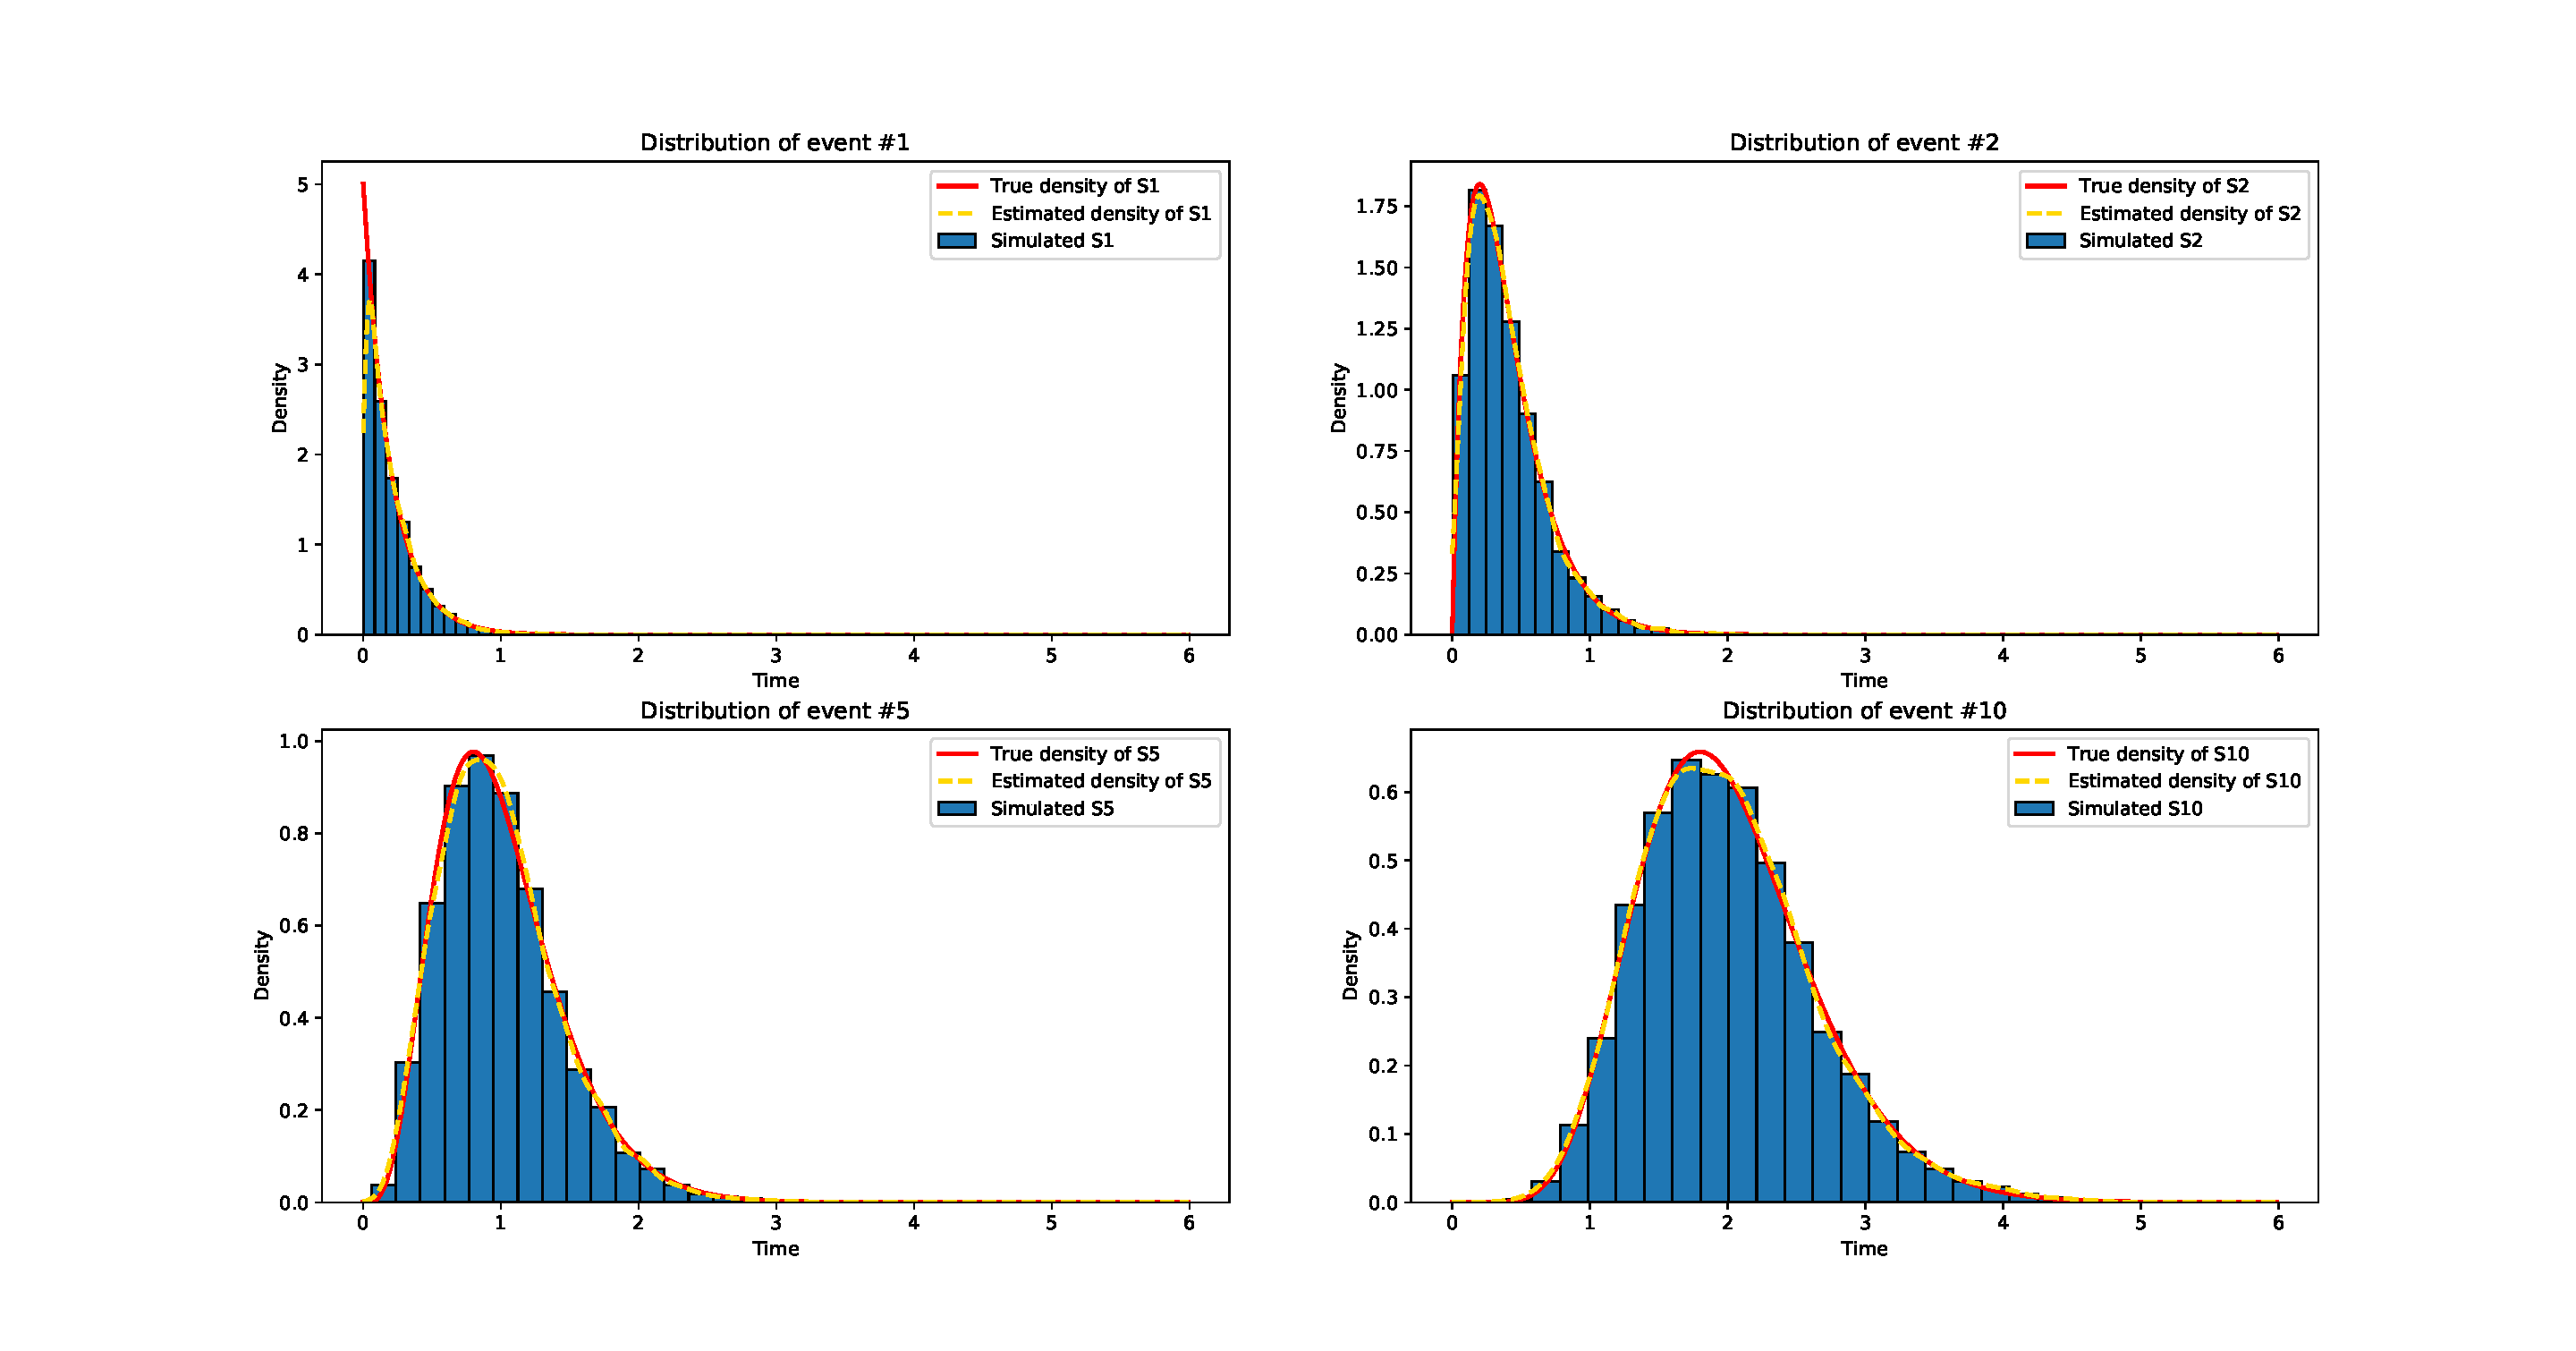
\includegraphics[width=\textwidth]{img/ex2.pdf}
\end{figure}

As we can see, the simulations agree with the theoretical distribution for each arrival time.\\
